\documentclass[a4paper, 10pt,onecolumn]{scrartcl}

%Standardpakete Deutsch
\usepackage[ngerman]{babel}
\usepackage[T1]{fontenc}
\usepackage[utf8]{inputenc}

%Extras
\usepackage{multirow}
\usepackage{natbib}
\usepackage{graphicx}
\usepackage{amsmath, amssymb}
\usepackage{graphicx}
\usepackage{grffile} %einfacheres einbinden von Dateipfaden
\usepackage{xpatch} %more space between title and subtitle
\usepackage{mathtools}
\usepackage{booktabs}
\newcommand{\changefont}[3]{
\fontfamily{#1} \fontseries{#2} \fontshape{#3} \selectfont}
\usepackage[export]{adjustbox}

\newlength{\myspace}
\setlength{\myspace}{2em}

\makeatletter
\xpatchcmd{\@maketitle}{\vskip.5em}{\vskip\myspace}{}{}
\makeatother

%\changefont{ptm}{m}{n}

\title{Computational Physics 1: Übung 8: Gekoppelte Differentialgleichungen - Nutzung von MatLab-Funktionen} 
\author{Jakob Hollweck} %auch nach \begindocument möglich
\setlength{\parindent}{0pt}
\date{Abgabe 02.02.18}

\begin{document}
\maketitle


\section*{Aufgabe 1: Ausbreitung eines Pulses}

Die Aufgabe war mithilfe der MatLab-Funktion ode45 das Runge-Kutta-Verfahren auf ein System von N=200 gekoppelten Oszillatoren anzuwenden, das pulsförmig durch  \[F_{ext}(t)=sin(\Omega t)\exp\left[
\frac{-(t-3T_0)^2}{T_0^2}
\right]
\] angeregt wurde. 
In Abbildung \ref{Abbildung1} ist nun die zeitliche Entwicklung der Gesamtenergie jedes Pendels des Systems dargestellt. Es ist gut zu erkennen, dass im Allgemeinen mit steigender Zeit die Energie eines Pendels abnimmt. Dies stimmt mit der Erwartung an ein gedämpftes System überein. 
Bei N=200 tritt nun ein Bereich hoher Energie auf, das Ende des gekoppelten Systems ist erreicht, der Gaußpuls wird reflektiert (was die hohe Energie erklärt), und interferiert mit den passierten Oszillatoren: Ein Prozess der insgesamt zu einer Dispersion des Pulses führt und so zu einem Auseinanderfließen der Energie. Beide Effekte traten schon vorher auf, nur nicht so stark. 
Das Prozess wiederholt sich bei N=1 mit niedrigerer Energie, wobei hier wieder eine Anregung durch die externe Kraft, die aber auch zeitlich abgenommen hat, erfolgt. Es kommt wieder zur Reflexion und Interferenz, diesmal auch mit der direkten Anregungsschwingung am ersten Pendel, was ein langwierigeres Interferenzmuster und breitere Dispersion zur Folge hat. Dies bedeutet ein weitere Verteilung der Energie und deutet die Konvergenz des gedämpften Systems an. Für t=500 ist eine nächste Reflexion bei N=200 zu erkennen: Da diese vorher bei t=200 auftrat, zeigt sich hier die verlangsamte Ausbreitungsgeschwindigkeit des Pulses mit der Zeit.

\begin{figure}[ht!]
	\centering
	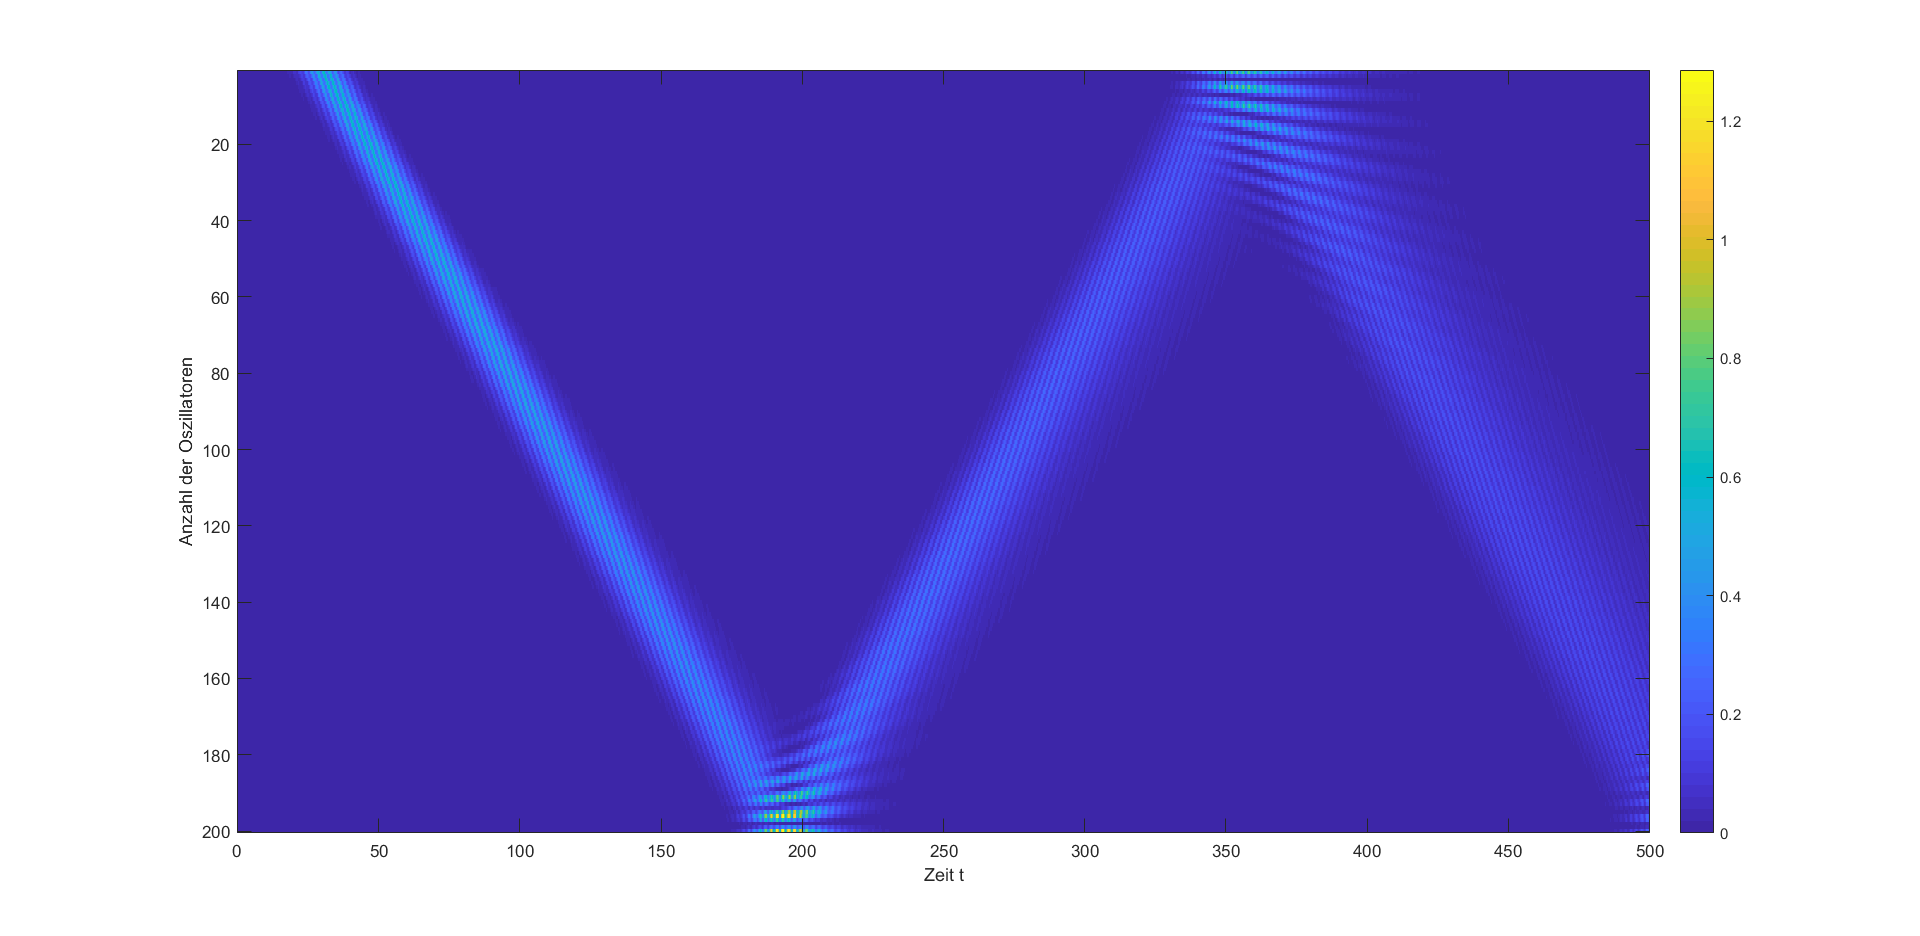
\includegraphics[scale=0.3,center]{En_Osz.png}
	\caption{Zeitliche Entwicklung der Gesamtenergie eines Pendels in einem System von 200 gekoppelten Oszillatoren.} 
	\label{Abbildung1}
\end{figure}


\end{document}